\documentclass{article}

\usepackage{hyperref}
\usepackage{xcolor}
\usepackage{amsmath}
\usepackage{mathtools}
\usepackage{graphicx}

\begin{document}

	\title{Leveraged Volume Sampling - Summary}
	\author{Ohad Ohayon}
	\pagenumbering{gobble}
	\maketitle
	\newpage

	\pagenumbering{arabic}

    \tableofcontents
    \newpage

    \section{Overview}
        This document summarises the contribution of the {\color{blue}\href{https://arxiv.org/abs/1802.06749}{\underline{paper}}} \textit{"Leveraged volume sampling for linear regression."}.
        It follows the structure of the paper itself, summarizing each of it's main sections.
        Finally, I will demonstrate my attempt at reproducing the results in the paper.

    \section{Introduction}
        \subsection{The Problem}
            Assume a linear regression problem where the feature vectors are the rows of an $n$ by $d$ full rank matrix $X=(x_{i}^T)$,
            the labels are the column vector $y$ and the optimal solution is $w^\ast=X^+y$.
            Define the average loss function of a solution $w$ to be $L(w)=\frac{1}{n}||Xw-y||_{2}^2$.
            In many real-world scenarios acquiring labels for some linear regression problems can be an expensive operation,
            although the regression features are readily available (as they may be just the parameters for an experiment).
            You may be accessible to the labels but you must limit the amount you request in order to deliver results within
            reasonable resource constraints.
            Assume the rows of such a sub-sampled problem to be $S$, the sub-sampled matrix and labels vector to be $X_{S}$
            and $y_{S}$ respectively and the sub-sampled solution to be $w_{S}^\ast=X_{S}^+y_{S}$.

            We'd like an effective algorithm to choose $S$, based on the features alone, whose corresponding solution $w_{S}^\ast$
            will hold the following properties with regard to the optimal solution $w^\ast$:
            \begin{itemize}
                \item $w_{S}^\ast$ is unbiased, i.e.: $E[w_{S}^\ast]=w^\ast$.
                \item The error for $w_{S}^\ast$ can be bounded by $L(w_{S}^\ast) < (1+\epsilon)L(w^\ast)$ for an $\epsilon$ of choice.
                \item Can be executed efficiently.
            \end{itemize}

            For the rest of this summary we'll assume $X$ is in general position unless otherwise specified.

        \subsection{Leverage Score Sampling}
            The leverage score $l_{i}$ of row $i$ of matrix $X=(x_{i}^T)$ is given by $l_{i}=x_{i}^T(X^TX)^{-1}x_{i}$ and those
            values sum up to $d$.
            \textit{Leverage Score Sampling} suggests selecting the multiset $S$ of $k$ rows i.i.d from $X$ with probability:

            \begin{equation}
                P(S\in{[n]^k})=\prod_{i=1}^{k}\frac{l_{i}}{d}
            \end{equation}

            With this procedure we are guaranteed\footnote{\label{leverage_score_performance_1}"Reverse iterative volume
            sampling for linear regression" P.21} that it is sufficient to choose
            $\mathcal{O}(d\log{d}+\frac{d}{\epsilon})$ to obtain $L(w_{S}^\ast) < (1+\epsilon)L(w^\ast)$ with high probability.
            All in all this is a pretty efficient and fast algorithm.
            However, this multiplicative bound doesn't hold in expectation and the approximate solution $w_{S}^\ast$ is biased (a
            trait of i.i.d sampling algorithms). This means that you can't control for the error by repeating the process
            and averaging the estimators.

        \subsection{Volume Sampling}
            Volume sampling is currently the main alternative to Leverage Score Sampling.
            It is a non-i.i.d sampling method that attempts to sample a "diverse" subset of the rows of $X$,
            where "diversity" is in the sense of trying to maintain as much of the volume spanned by the
            columns of $X$.
            \textit{Volume Sampling} suggest selecting the set $S$ of $k$ distinct rows from $X$ with the following probability:

            \begin{equation}
                P(S\in{\binom{[n]}{k}})=\frac{det(X_{S}^TX_{S})}{\binom{n-d}{k-d}det(X^TX)}
            \end{equation}

            This resultant $w_{S}^\ast$ is unbiased, which in turn allows the averaging of multiple results to reduce the variance.
            This procedure can also be implemented efficiently using the \textit{"Reverse Iterative Sampling"} and \textit{"Fast Regularized
            Volume Sampling"} {\color{blue}\href{https://arxiv.org/abs/1710.05110}{\underline{algorithms}}}\footnote{\label{reg_vol_samp}"Subsampling
            for Ridge Regression via Regularized Volume Sampling"}.
            However, there is no high probability guarantee of a $(1+\epsilon)L(w^\ast)$ bound on $L(w_{S}^\ast)$ for this procedure
            (as shown in \hyperref[sec:no_mult_bound_vol]{the following section}).

        \subsection{Leveraged Volume Sampling}
            \textit{Leveraged Volume Sampling} is this paper's contribution and it defines an unbiased sampling procedure with high probability
            guarantees of multiplicative bounds for a relatively small $k$.
            The procedure suggests sampling $k$ lines from $X$ with repetition in the following proportion:

            \begin{equation}
                P(\pi\in{[n]^k}) \propto det(\sum_{i=1}^{k}\frac{d}{l_{\pi_{i}}}x_{\pi_{i}}x_{\pi_{i}}^T)\prod_{i=1}^{k}\frac{l_{\pi_{i}}}{d}, \text{where } l_{i}=x_{i}^T(X^TX)^{-1}x_{i}
            \end{equation}

    \section{No Multiplicative Bound For Standard Volume Sampling}
        \label{sec:no_mult_bound_vol}
        First, the paper first demonstrates that for the following $n x d$ regression problem:
        \begin{equation*}
            X=
                \begin{bmatrix}
                    I_{dxd} \\
                    \gamma I_{dxd} \\
                    \vdots \\
                    \gamma I_{dxd}
                \end{bmatrix}
            , y=
                \begin{bmatrix}
                    1_{dxd} \\
                    0_{d} \\
                    \vdots \\
                    0_{d}
                \end{bmatrix}
            , \text{where } \gamma > 0
        \end{equation*}

        The paper proves that if $S$ of size $k$ is picked via ordinary \textit{Volume Sampling} then the following holds:
        \begin{equation}
            \lim\limits_{\gamma \to 0} \frac{E(L(w_{S}^\ast))}{L(w^\ast)} \geq 1+\frac{n-k}{n-d}
        \end{equation}
        \begin{equation}
            \exists \gamma > 0: \forall k \leq \frac{n}{2}: P(L(w_{S}^\ast) \geq (1+\frac{1}{2})L(w^\ast)) > \frac{1}{4}
        \end{equation}

        This means that for \textit{Volume Sampling}:
        \begin{itemize}
            \item There can be no unconditional guarantee on the unbiasedness of the loss $L(w_{S}^\ast)$.
            \item There can be no unconditional upper bound guarantee with high probability on the required $k$ which is less than $\mathcal{O}(n)$.
        \end{itemize}

        \textit{Leveraged Volume Sampling} does away with these limitations.

    \section{Rescaled Volume Sampling Analysis}
        \textit{Leveraged Volume Sampling} is a specific case of \textit{Rescaled Volume Sampling}.
        Assume:
        \begin{equation*}
            \forall 1 \leq i \leq n: 0 \le q_{i} \leq 1, \text{ and } \sum_{i=1}^{n}q_{i} = 1
        \end{equation*}
        Then $(q_{i})_{i=1}^n$ defines a distribution over the lines of $X$.
        \textit{Rescaled Volume Sampling} suggests sampling $k$ rows with repetition from $X$ with the following proportion:
        \begin{equation}
            P(\pi \in [n]^k) \propto det(\sum_{i=1}^{k}\frac{1}{q_{\pi_{i}}}x_{\pi_{i}}x_{\pi_{i}}^T)\prod_{i=1}^{k}q_{\pi_{i}} = det(X^{T}Q_{\pi}X)\prod_{i=1}^{k}q_{\pi_{i}},
            \text{ where } Q=\sum_{i=1}^{k}\frac{1}{q_{\pi_{i}}}e_{\pi_{i}}e_{\pi_{i}}^T
        \end{equation}
        \begin{equation}
            w_{\pi}^\ast=(Q_{\pi}^{1/2}X)^{+}Q_{\pi}^{1/2}y
        \end{equation}

        By application of the following theorems the paper proves that $w_{\pi}^\ast$ is unbiased:
        \begin{itemize}
            \item The Cauchy-Binet theorem, decomposing $det(XQ_{\pi}X)$ as the sum of determinants of square sub-matrices of $X$, to calculate $\sum_{\pi \in [n]^k}det(X^{T}Q_{\pi}X)\prod_{i=1}^{k}q_{\pi_{i}}$.
            \item $E((I_{S}X)^+) = X^+$ for ordinary volume sampling to decompose both $w_{\pi}^\ast$ and $w^\ast$.
        \end{itemize}

        Furthermore, using a bit of algebra, the paper shows that for \textit{Rescaled Volume Sampling}:
        \begin{equation}
            E(Q_{\pi}) = (k-d)I + diag(\frac{l_{1}}{q_{1}}, \hdots, \frac{l_{n}}{q_{n}})
        \end{equation}

    \section{Leveraged Volume Sampling}
        \textit{Leveraged Volume Sampling} is \textit{Rescaled Volume Sampling} where $q_{i}=\frac{l_{i}}{d}$ (note that $\sum_{i=1}^{n}l_{i}=d$).
        This procedure is unbiased (as it is a case of \textit{Rescaled Volume Sampling}) and is subject to favorable tail bounds (more on that in the next section).
        You can poll such a subset with an algorithm named \textit{Determinantal Rejection Sampling} which selects $k$ lines from $X$ that boils down to the following steps:
        \begin{itemize}
            \item Set $s \coloneqq max(k, 4d^{2})$.
            \item Repeat until acceptance selection of lines $\pi$ of size $s$ i.i.d from $1..n$ and accept with probability $\frac{det(\frac{1}{s}X^{T}Q_{\pi}X)}{det(X^{T}X)}$.
            \item Use \textit{Volume Sampling} to reduce the selected $s$ rows to $k$ rows.
        \end{itemize}

        The proof that this procedure indeed yields a \textit{Leveraged Volume Sampling} distributed set is largely due to the fact that when you
        select a \textit{Leveraged Volume Sampling} distributed set of size $s$ and then apply \textit{Reverse Iterative Volume Sampling} to sub-select
        a $k$ sized subset then the \textit{Leveraged Volume Sampling} distribution is recursively maintained at each step.

        This algorithm runs, with probability at least $1-\delta$, in time $\mathcal{O}((d^2+k^2)d^2ln(\frac{1}{\delta}))$.
        This can be seen by bounding from below the acceptance probability in the repetition with $\frac{3}{4}$ and noting that determinant
        calculation takes at most as much as decomposing a matrix via SVD which is $\mathcal{O}(sd^2)$.
        Finally, note that $s=\mathcal{O}(k+d^2)$.

    \section{Tail Bounds For Leveraged Volume Sampling}
        To analyze tail bounds the paper shifts to assesing the problem where instead of $X=(x_{i}^T)_{i=1}^{n}$ you have an orthogonal $U=(u_{i}^T)_{i=1}^{n}, U^TU=I$ that spans the range.
        This maintains correctness due to the following properties:
        \begin{itemize}
            \item The leverage scores are equal: $\forall i: x_{i}^T(X^TX)^{-1}x_{i}=u_{i}^T(U^TU)^{-1}u_{i}$
            \item The \textit{Volume Sampling} volumes are proportional: $\forall S: det(X_{S}^TX_{S}) \propto det(U_{S}^TU_{S})$
            \item The \textit{Leveraged Volume Sampling} volumes are proportional: $\forall \pi: det(X^TQ_{\pi}X) \propto det(U^TQ_{\pi}U)$
        \end{itemize}

        The following notation changes hold:
        \begin{itemize}
            \item $v^\ast=argmin||Uv - y||$
            \item $v_{\pi}^\ast=argmin||U_{\pi}v - y_{\pi}||$
            \item $L(v) = ||Uv - y||, L(v^\ast) = L(w^\ast), L(v_{\pi}^\ast) = L(w_{\pi}^\ast)$
            \item $r \coloneqq Uv^\ast - y, U^Tr = 0$
        \end{itemize}

        Obtaining a multiplicative bound on $L(v_{\pi}^\ast)$ is done by reducing the problem to:
        \begin{equation}
            ||v_{\pi}^\ast - v^\ast|| \leq ||(U^TQ_{\pi}U)^{-1}||||U^TQ_{\pi}r||
        \end{equation}
        And bounding these two factors.
        By the following two traits we can get a multiplicative bound of $L(w_{\pi}^\ast) < (1+\epsilon)L(w^\ast)$,
        with high probability, when $k=\Omega(d\log \frac{d}{\delta} + \frac{d}{\epsilon\delta})$:
        \begin{itemize}
            \item if $k \geq \frac{2d}{\epsilon}$ then $E(||\frac{1}{k}U^TQ_{\pi}r - U^Tr||^2) \leq \epsilon||r||^2$
            \item There exists a $C$ s.t. if $k \geq Cd\log(\frac{d}{\delta})$ then $P(\lambda_{min}(\frac{1}{k}U^TQ_{\pi}U) \leq \frac{1}{8}) \leq \delta$
        \end{itemize}

        To prove the first property, the paper demonstrates:
        \begin{equation}
            E(||\frac{1}{k}U^TQ_{\pi}r - U^Tr||^2) = r^TE((\frac{1}{k}Q_{\pi}-I)UU^T(\frac{1}{k}Q_{\pi}-I))r \leq ||E((\frac{1}{k}Q_{\pi}-I)UU^T(\frac{1}{k}Q_{\pi}-I))||||r||^2
        \end{equation}
        And proceeds to bound $||E((\frac{1}{k}Q_{\pi}-I)UU^T(\frac{1}{k}Q_{\pi}-I))||$ via a clever application of a Hadamard Product inequality.

        The first property, when applied to $r=Uv^\ast - y$, allows us to bound $||U^TQ_{\pi}r||^2 \leq \epsilon\frac{k^2}{8^2}||r||^2$
        and the second allows us to bound $||(U^TQ_{\pi}U)^{-1}|| < 8$, both with high probability, there by yielding the bound:
        \begin{equation}
            L(w_{\pi}^\ast) \leq (1+\epsilon)L(w^\ast)
        \end{equation}

    \newpage
    \section{Numerical Results}
        I've done my best to replicate the results in the paper.
        The trend of diminishing error at relatively small number of rows is there but I couldn't replicate the smooth results the paper presented.

        \begin{figure}[h]
            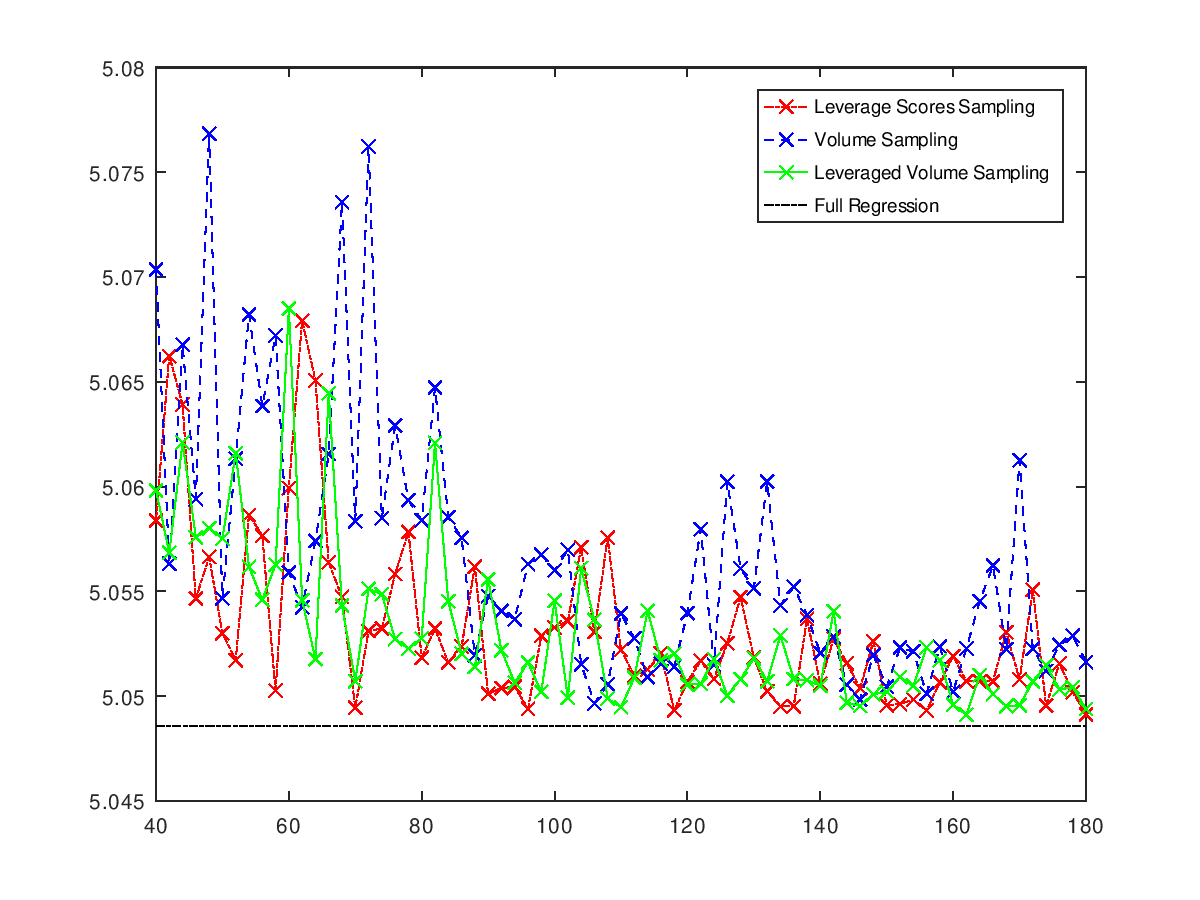
\includegraphics[width=\linewidth]{results/abalone.png}
            \caption{abalone dataset.}
            \label{fig:dataset1}
        \end{figure}
        \begin{figure}[h]
            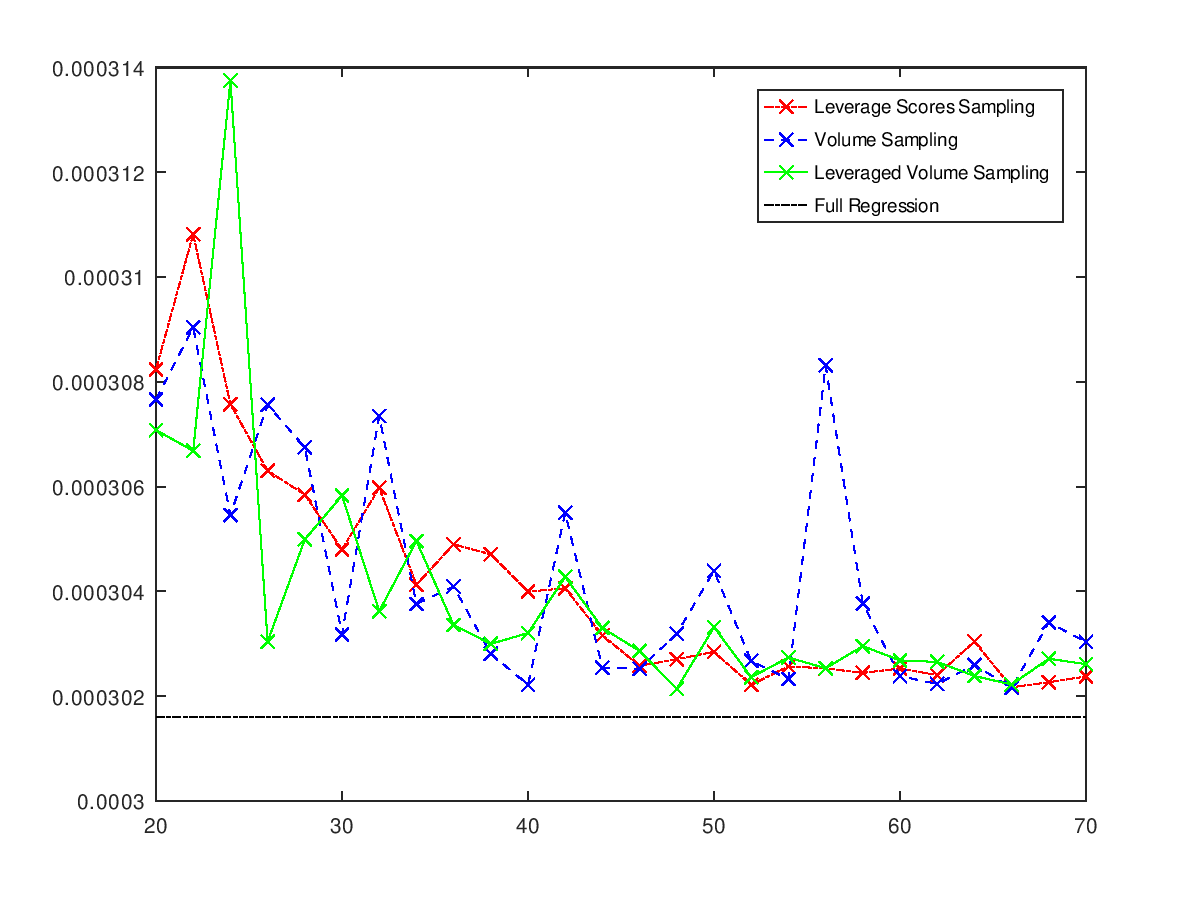
\includegraphics[width=\linewidth]{results/bodyfat.png}
            \caption{bodyfat dataset.}
            \label{fig:dataset1}
        \end{figure}
        \begin{figure}[h]
            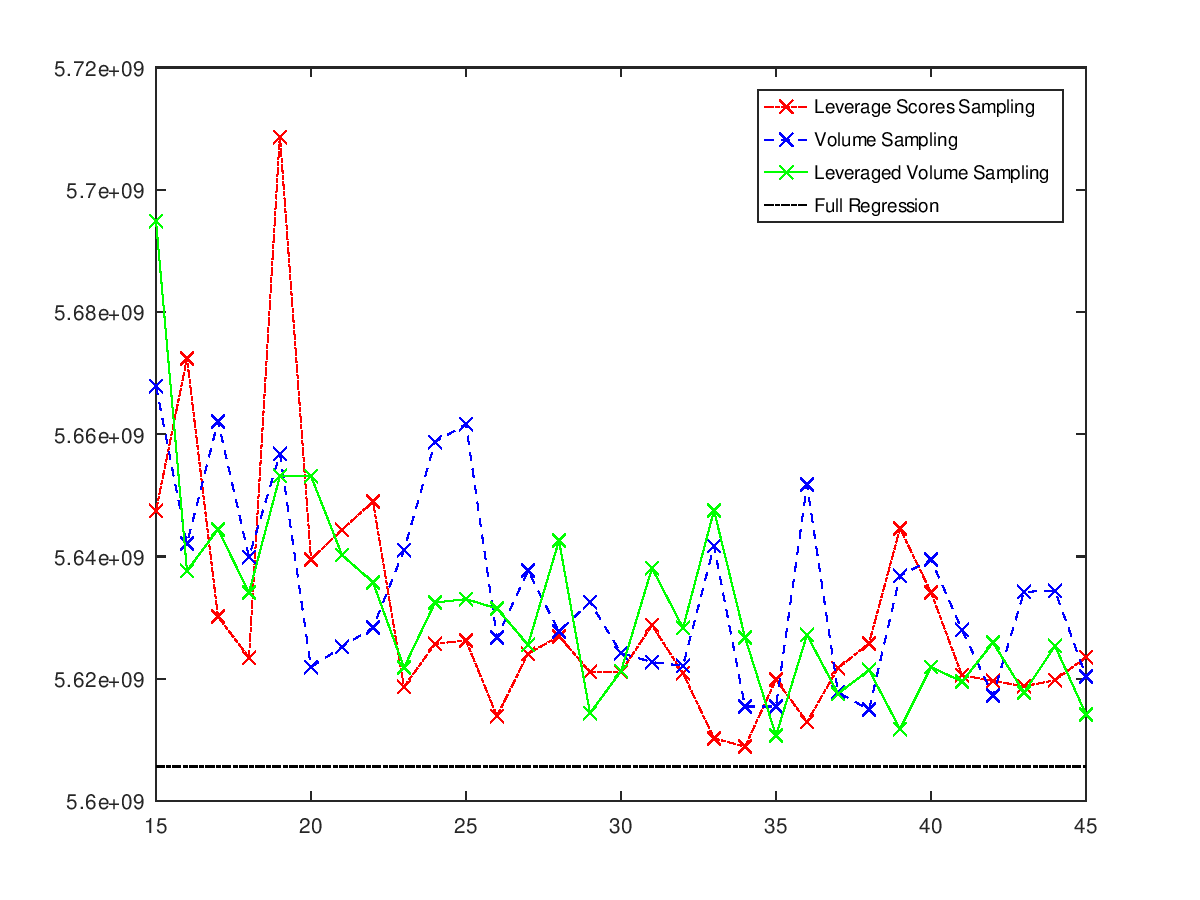
\includegraphics[width=\linewidth]{results/cadata.png}
            \caption{cadata dataset.}
            \label{fig:dataset1}
        \end{figure}
        \begin{figure}
            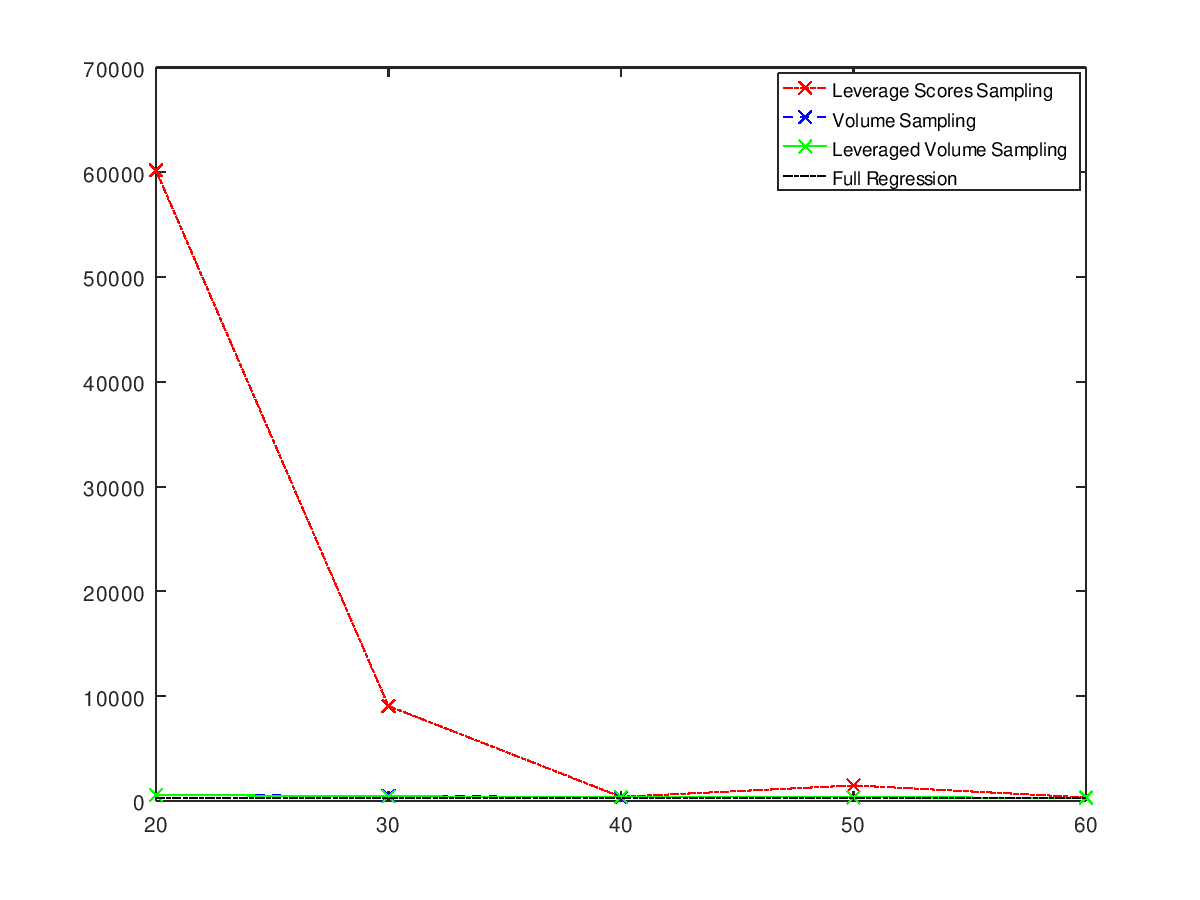
\includegraphics[width=\linewidth]{results/cpusmall.png}
            \caption{cpusmall dataset.}
            \label{fig:dataset1}
        \end{figure}
        \begin{figure}
            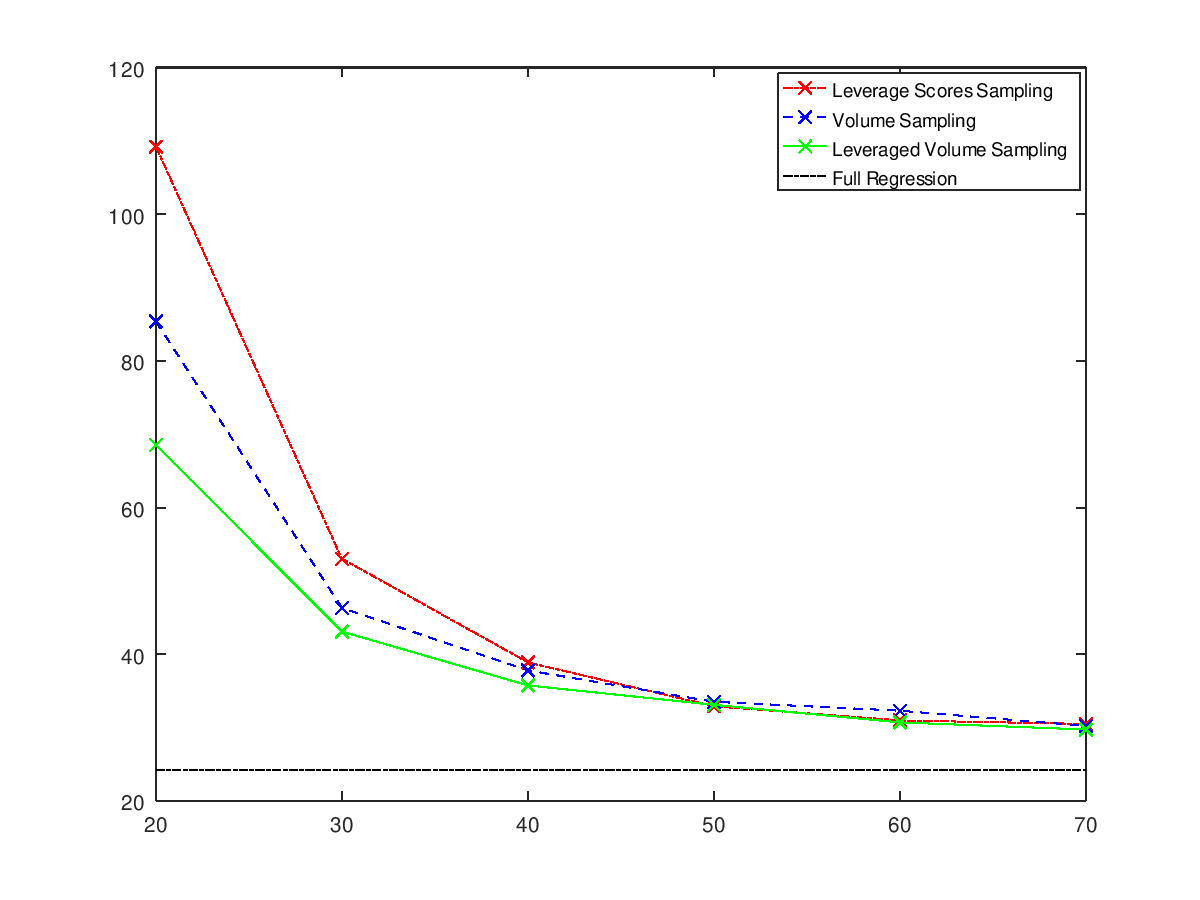
\includegraphics[width=\linewidth]{results/housing.png}
            \caption{housing dataset.}
            \label{fig:dataset1}
        \end{figure}
        \begin{figure}
            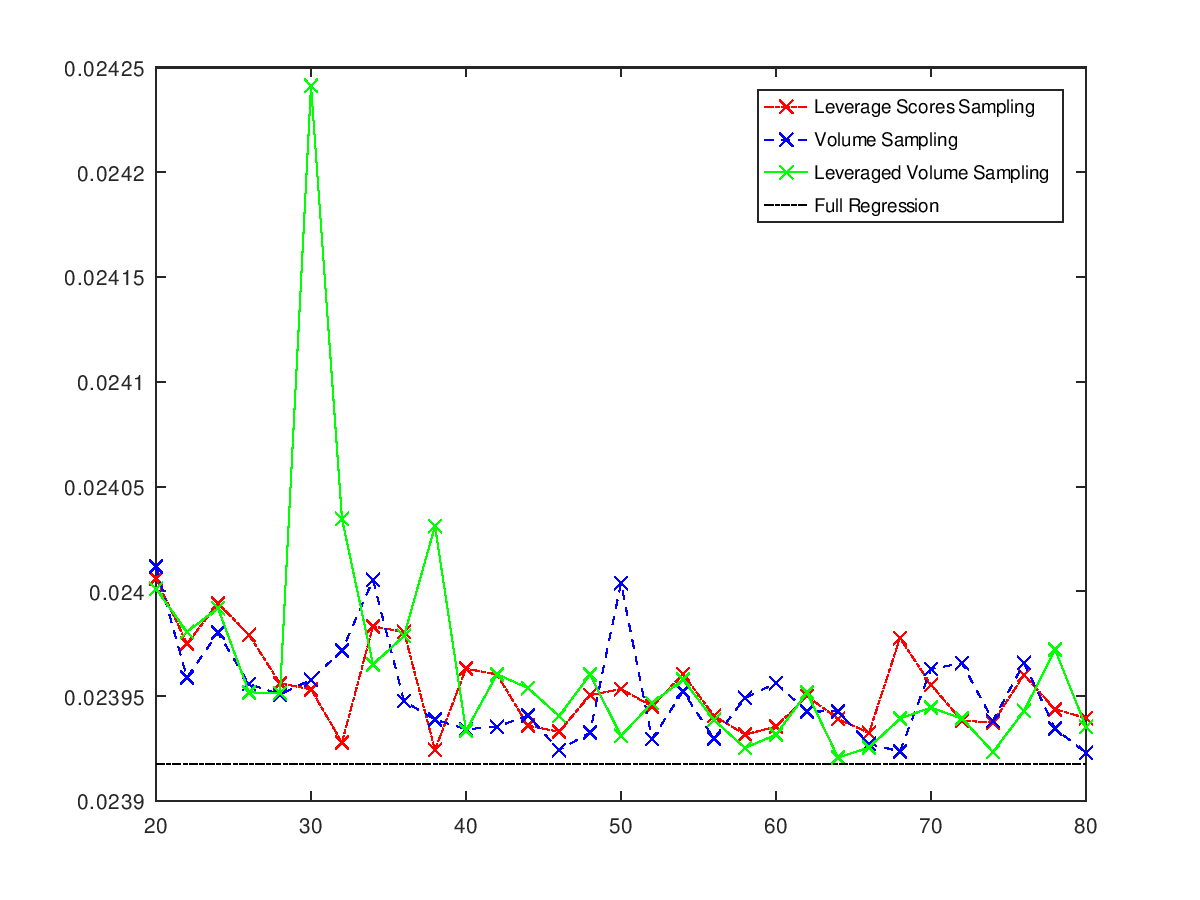
\includegraphics[width=\linewidth]{results/mg.png}
            \caption{mg dataset.}
            \label{fig:dataset1}
        \end{figure}

\end{document}

